% !TEX root = ../main.tex

%************************************************
\chapter{Introduction}
\label{ch:intro}
%************************************************

%There are also a very small number of BALQSOs with redshifted absorption

% http://adsabs.harvard.edu/abs/2013MNRAS.434..222H

In $1963$, the powerful radio source $3$C $273$ was identified with a star-like, thirteenth magnitude object with a strongly redshifted ($z=0.158$) optical spectrum \citep{schmidt63}. 
Assuming this redshift was due to the Hubble expansion of the Universe, this finding implied $3$C $273$ was at an enormous distance ($500$ megaparsecs) and was $10$ times brighter than the most luminous galaxies. 
Variability on time-scales of weeks suggested that the source was very compact (i.e. smaller than a light-week).
It was quickly realised that `quasars'\footnote{The term `quasar' originated as a contraction of `quasi-stellar radio source', although 90 per cent of quasars are now known to be radio-quiet.}, and other lower-luminosity classes of active galactic nuclei (AGN)\footnote{Throughout this thesis we use the terms `quasar' and `Active Galactic Nucleus (AGN)' interchangeably to describe active super-massive black holes, although the term quasar is generally reserved for the luminous (L$_{\mathrm Bol} > 10^{12}{\mathrm L}_{\odot}$) subset of AGNs.}, are powered by the release of gravitational potential energy as mass is accreted onto a super-massive\footnote{Super-massive: $10^{6 - 9}$ M$_\odot$.} black hole (BH) at the centre of a galaxy \citep[e.g.][]{hoyle63,salpeter64,lynden-bell69,lynden-bell71}. 

Begining in the early $1990$s, inactive super-massive BHs were found in the centres of many nearby massive galaxies \citep[e.g.][]{kormendy95,ferrarese05,kormendy13}.
This proved that quasar activity is a stage in the life of all massive galaxies \citep[e.g.][]{lynden-bell69}. 
Shortly after, it was discovered that the BH mass and the properties of the host-galaxy bulge were strongly correlated \citep[e.g. the BH mass and the stellar velocity dispersion in the host galaxy bulge, M$_{\mathrm BH}$-$\sigma$;][]{ferrarese00,gebhardt00,graham01,tremaine02,marconi03,aller07,gultekin09}.
This was an unexpected finding, given that the sphere-of-influence\footnote{Sphere-of-influence: where the gravity of the BH dominates over the other mass components.} of a BH, $\lesssim100$ parcsecs \citep[e.g.][]{kormendy13}, is many orders of magnitude smaller than a typical galactic bulge. 
It suggests that the BH and the host galaxy bulge grow synchronously, with the energetic output of the rapidly-accreting BH coupling with the gas in the host galaxy and regulating star formation and the growth of the BH itself \citep[e.g.][]{silk98,king03,dimatteo05,king15}. 

The number density of quasars, which evolves strongly with redshift, peaks at redshifts $2 \lesssim z \lesssim 3$ \citep[e.g.][]{brandt05,richards06b} and the most massive (M$_{\mathrm BH} \gtrsim 10^9\msun$) present-day BHs experienced much of their growth during this epoch.  
The cosmic star formation rate history closely follows the cosmological evolution of the quasar luminosity function \citep[e.g.][]{boyle98}, which establishes a further connection between BH and galaxy properties.
Quasar feedback has also been invoked to reproduce the high-mass end of the galaxy luminosity function in cosmological simulations \citep[e.g.][]{kauffmann00}.
The insight that quasars may play a crucial role in the evolution of galaxies has led to an explosion of interest in their properties in recent years. 

\section{AGN: current paradigm}

\begin{figure}
  \centering
  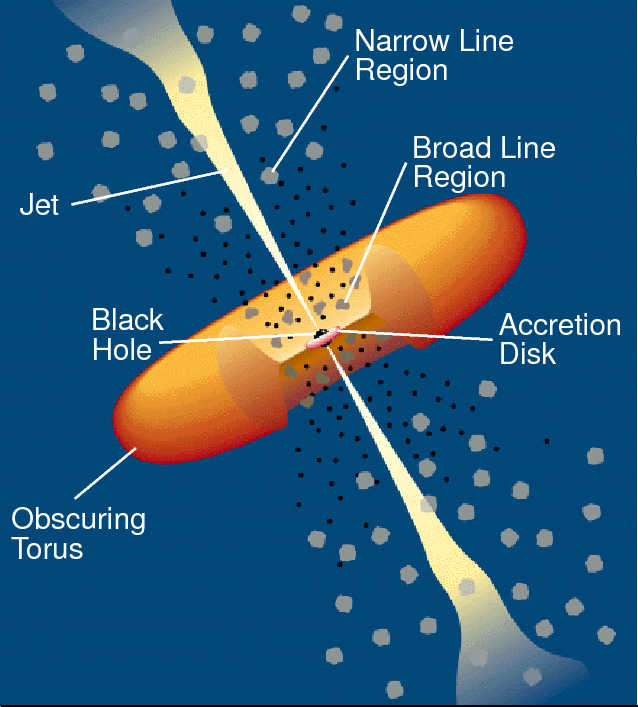
\includegraphics[width=0.5\textwidth]{figures/chapter05/urry_model}
  \caption[{Illustration of the physical structure of an AGN in a simple orientation-based unification model.}]{Cartoon picture of the inner regions on an AGN. Credit: \citet{urry95}.}
  \label{fig:agnmodel}
\end{figure}

The basic features of the current AGN paradigm are widely accepted, although many of the details are unknown. 
The basic features are: a hot accretion disc surrounding a super-massive BH, rapidly orbiting clouds of ionised gas, and a dusty, obscuring structure (generally referred to as the `torus'). 
Collimated jets of relativistic plasma and/or associated lobes are also seen in the $10$ per cent of quasars that are radio-loud \citep[e.g.][]{peterson97}. 
A cartoon picture illustrating the basic structure of an AGN is shown in Figure~\ref{fig:agnmodel}. 

\subsection{Accretion disc}

Material is pulled towards a super-massive BH and sheds angular momentum through viscous and turbulent processes in a hot accretion disc \citep[e.g.][]{begelman85}. 
The accretion disc reaches temperatures of $\sim10^6$ K, and radiates primarily at ultraviolet (UV) to soft-X-ray wavelengths. 

\subsection{The broad line region}

One of the pre-eminent features of many AGN spectra are broad optical and UV emission lines produced in the broad line region (BLR). 
The BLR consists of gas clouds at distances from several light-days to several light-months that are photo-ionised by the ultraviolet continuum emission emanating from the accretion disc.  
Because of the close proximity to the central super-massive BH, bulk motions are dominated by gravity and radiation pressure from the accretion disc.
The very broad emission line widths are assumed to Doppler-broadened, and imply line-of-sight velocities of many thousands of\,\kms. 

\subsection{The dusty torus}

Further out from the central engine are dusty, molecular clouds which are co-planar with the accretion disc. 
These dusty clouds are generally referred to as the `torus'. 
In a Type II AGN, the system is observed in an edge-on configuration and, as a result, emission from the accretion and BLR is obscured by the dusty torus \citep[e.g.][]{antonucci93}.
Although this simple picture (shown in Figure~\ref{fig:agnmodel} as well as in countless other publications) is a useful starting point, the idea of a torus as a static, doughnut-like structure is almost certainly incorrect. 
For example, the problem of maintaining the large scale height required to explain the observed fraction of Type $1$/$2$ AGN has long been recognized \citep[e.g.][]{krolik88}. 
In one set of models, the torus is the dusty part of an accretion disc wind that extends beyond the dust-sublimation radius \citep[e.g.][]{konigl94,everett09,gallagher12,everett05,keating12,elitzur06}. 

\subsection{The narrow line region}

Further away from the central BH and beyond the dusty torus is the narrow emission line region (NLR). 
Like the BLR, the NLR is ionised by radiation from the accretion disc. 
Unlike the BLR, densities in the NLR are low enough that forbidden transitions are not collisionally suppressed. 
Emission line widths are typically hundreds of\,\kms\, in the NLR. 

\section{Winds and outflows in AGN}

Quasars are very powerful sources of radiation, and are embedded in matter-rich environments at the centres of galaxies.
Strong winds, driven by some combination of gas pressure, radiation pressure, and magnetic forces, are to be expected under these conditions \citep[e.g.][]{blandford82b,proga00,everett05}. 
In line with these expectations, evidence for outflowing gas is common in the spectra of quasars. 

Perhaps the most dramatic evidence of outflows is seen in broad absorption line quasars \citep[BALQSOs;][]{weymann91}.
BALQSOs are characterised by broad absorption features in the ultra-violet resonance lines of highly ionised \ion{N}{V}, \ion{C}{IV} and \ion{Si}{IV}. 
The absorption troughs are thousands of\,\kms\, wide and at large blueshifts relative to the quasar rest-frame\footnote{Much rarer cases of redshifted BAL troughs do also exist \citep[e.g.][]{hall13}.}. 
The absorption is thought to occur in outflows reaching $60\,000$\,\kms\, \citep[e.g.][]{turnshek88}. 
The far-side of the outflow is obscured by the accretion disc, and so only the near-side, which is moving towards the observer, is detected. 
The observed \ion{C}{IV} BALQSO fraction in radio-quiet quasars is $\sim15$ per cent \citep[e.g.][]{hewett03,reichard03} and the intrinsic fraction in the quasar population has been estimated at $\sim40$ per cent \citep{allen11}.
Outflows can also explain narrow UV and X-ray absorption lines (NALs) which are seen in $\sim60$ per cent of Seyfert 1 galaxies\footnote{Seyfert 1: A class of AGN with broad emission lines and clearly detectable host galaxies.} \citep{crenshaw99} and some quasars \citep[e.g.][]{hamann97}. 

The blueshifting of high-ionisation lines in the BLR (including \ion{C}{IV}) can be understood if the lines are produced in outflowing clouds (although see, e.g., \citealt{gaskell16}, for an alternative explanation). 
The blueshifting of \ion{C}{IV} appears to be nearly ubiquitous in the quasar population \citep[e.g.][]{richards02,richards11}. 

Together, these results suggest that outflows are very common and the energy released by quasars can have a dramatic effect on their immediate surroundings. 
Accretion-disc wind models have been developed to explain the wide range of emission and absorption line phenomena described above \citep[e.g.][]{murray95,elvis00,proga00,everett05}.
UV photons excite the partially-ionised material surrounding the accretion disc. 
This exerts a pressure on the atoms - a phenomenon known as radiation line-driving - and a wind is blown from the accretion disc. 
  
In models for the co-evolution of quasars and galaxies, the energy released by quasars impacts galaxies on much larger scales than is probed by the emission and absorption diagnostics described above.  
In recent years, a huge amount of resources have been devoted to searching for observational evidence of galaxy-wide, quasar-driven outflows \citep[for recent reviews, see][]{alexander12,fabian12,heckman14}.
This has resulted in recent detections of outflows in AGN-host galaxies using tracers of atomic, molecular, and ionised gas with enough power to sweep their host galaxies clear of gas \citep[e.g.][]{nesvadba06,arav08,nesvadba08,moe09,dunn10,alexander10,harrison12,harrison14,nesvadba10,rupke13,veilleux13,nardini15,feruglio10,alatalo11,cimatti13,cicone14}.  

\section{Measuring black hole masses}

The BH mass is one of the most important physical parameters of a quasar and considerable resources have been devoted to measuring the masses of BHs in active galaxies. 
Large-scale studies of AGN and quasar demographics have become possible through the calibration of single-epoch virial-mass estimators using BH masses from reverberation-mapping \citep[e.g.][]{peterson10,vestergaard11,marziani12,shen13}.  

\subsection{Reverberation mapping}

Under the assumptions that the BLR dynamics are virialised\footnote{The virial theorem states that the average kinetic energy of a system is equal to half of the average negative potential energy.} and the gravitational potential is dominated by the BH, the BH mass is given by:

\begin{equation}
M_{\mathrm BH} \simeq \frac{V_{\mathrm Virial}^2R_{\mathrm BLR}}{G} 
\end{equation}

where $V_{\mathrm virial}$ is the virial velocity in the BLR and $R_{\mathrm BLR}$ the characteristic BLR radius.
The problem of measuring the mass therefore reduces to the problem of measuring the velocity and orbital radius of the line-emitting clouds in the BLR. 

Continuum variability is a common characteristic of quasars, owing to the stochastic nature of the accretion process.  
Because the BLR is photo-ionized by the continuum, the broad emission lines also vary with some characteristic lag, which is related to the light travel time across the BLR. 
The reverberation mapping method, first proposed by \citet{blandford82a}, uses the time lag between variations in the continuum emission and correlated variations in the broad line emission to measure the typical size of the BLR \citep[e.g.][]{peterson93,netzer97,peterson14}. 

The typical velocity in the BLR is measured from the Doppler-broadened width of an emission line produced in the BLR. 
Since the structure and geometry of the BLR is unknown, a virial coefficient, $f$, is introduced to transform the observed line-of-sight velocity inferred from the line width in to a virial velocity.
Unfortunately, $f$ is unknown and likely varies from object to object.  
In practice, the value of $f$ is empirically determined by requiring that the reverberation-mapping masses are consistent with those predicted from the M$_{\mathrm BH}$-$\sigma$ relation for local inactive galaxies. 

Because reverberation mapping depends on temporal resolution rather than spatial resolution, this technique can be applied out to much greater distances than direct dynamical modelling \citep[e.g.][]{kormendy13}.
However, because reverberation mapping relies on dense spectrophotometric monitoring campaigns which span many years, the number of AGN with measured lags is limited to $\sim50$ AGN \citep[e.g.][]{kaspi00,peterson04,kaspi07,bentz09,denney10,barth11,grier12}. 
This sample is strongly biased to low luminosity Seyfert $1$ galaxies, and the maximum redshift is just $z\sim0.3$. 
Comprehensive statistical studies of active BHs, particularly during the epoch of peak galaxy formation ($z\gtrsim2$), therefore require a different approach to measuring BH masses. 

\subsection{Single-epoch virial estimates}

Reverberation mapping campaigns have also revealed a tight relationship between the radius of the BLR and the quasar optical (or ultraviolet) luminosity \citep[the ${\mathrm R_{BLR}-L}$ relation; e.g.][]{kaspi00,kaspi07}.
A slope of $\simeq0.5$ is found, which is consistent with naive predictions \citep[e.g.][]{peterson97}. 
This relation provides a much less expensive method of measuring the BLR radius, and large-scale studies of AGN and quasar demographics have thus become possible through the calibration of single-epoch virial-mass estimators \citep[e.g.][]{vestergaard02,mclure02,vestergaard06,mcgill08,wang09,rafiee11,park13}.
Single-epoch virial BH mass estimates normally take the form

\begin{equation}
  \label{eq:virialmass}
  \mathrm{M_{BH}} = 10^{a} \left( \frac{\Delta V}{1000~\mathrm{km~s^{-1}}} \right)^b \left( \frac{L_{\lambda}}{10^{44}~\mathrm{erg~s^{-1}}} \right)^c
\end{equation}

\noindent where $\Delta V$ is a measure of the line width, $L_\lambda$ is the monochromatic continuum luminosity at wavelength $\lambda$, and $a$, $b$, and $c$ are coefficients, determined via calibration against a sample of AGN with reverberation-mapping BH mass estimates. 

Virial BH masses have made possible large-scale studies of AGN and quasar demographics \citep[e.g.][]{greene05b,vestergaard06,vestergaard09,shen11,shen12,trakhtenbrot12}. 
With these masses, the growth rate of massive BHs can be measured across cosmic time. 
This conveys important information about the accretion processes occuring in active BHs \citep[e.g.][]{kollmeier06} and is crucial in order to understand the processes responsible for establishing the M$_{\mathrm BH}$-$\sigma$ relation \citep[e.g.][]{bennert11}.
Single-epoch virial estimates have been used to calculate BH masses in the highest redshift quasars \citep[e.g. a $10^9$M$_\odot$ BH in a redshift $z\sim7$ quasar;][]{mortlock11}. 
The fact that a $10^9$M$_\odot$ BH exits when the age of the Universe is less than $1$ Gyr places tight constraints on its accretion history \citep[e.g.][]{willott03}. 

The uncertainties in reverberation mapped BH masses are estimated to be $\sim 0.4$ dex \citep[e.g.][]{peterson10}, and the uncertainties in virial masses are similar \citep[e.g.][]{vestergaard06}.
However, the main concern and biggest unknown is the extension of the method to high redshifts. 
This requires that the relations calibrated for sub-Eddington BHs with M$\sim10^7$ are valid for BHs with masses up to $10^{10}$ that are radiating near the Eddington limit. 
Furthermore, the vast majority of these measurements are done using \hbns, and so the $R-L$ relation has been established using \hbns.
\hb is redshift beyond the reach of optical spectrographs at $z \gtrsim XX$, and extending the method to higher redshifts requires the secondary-calibration of other low-ionization emission lines such as \ha ($6564.6$\AA) and \ion{Mg}{II}\ll$2796.4$,$2803.5$ \citep[e.g.][]{vestergaard02,mclure02,wu04,kollmeier06,onken08,wang09,rafiee11}.
At redshifts $z \gtrsim 2$, only the high-ionisation \ion{C}{IV} emission line is available, but many authors have reported \ion{C}{IV}-based masses to be inconsistent with masses based on other lines. 
These issues are explored in detail in Chapter~\ref{ch:bhmass}.

\section{The advent of large surveys}

The Palomar-Green (PG) Bright Quasar Survey \citep[BQS;][]{schmidt83}, the first large-area quasar survey, identified $114$ quasars via their UV excess. 
\citet{boroson92} were among the first to use this large sample to analyse quasar spectroscopic properties in a systematic way.
With the advent of CCD technology came a new generation of surveys, most notably the Sloan Digital Sky Survey \citep[SDSS;][]{york00} and the $2$QZ survey \citep{croom04}. 
SDSS, and the next-generation Baryon Oscillation Spectroscopic Survey \citep[BOSS;][]{dawson13}, now contain spectra of $\sim300\,000$ AGN and quasars. 

These large, uniform data sets have revolutionised the study of AGNs and quasars by facilitating statistical studies of the properties of quasars and AGNs covering wide ranges in redshift and luminosity. 
This has greatly enhanced our understanding of AGNs and their connections to their host galaxies, especially when combined with multi-wavelength coverage. 
This has been achieved in recent years with sensitive, wide-field photometric surveys, including the UV/optical SDSS, the near-infrared UKIRT Infrared Deep Sky Survey \citep[UKIDSS;][]{lawrence07} and the mid-infrared Wide-field Infrared Explorer \citep[WISE;][]{wright10}.  

\section{Overview of thesis}

\subsection{Chapter 1: A near-infrared spectroscopic database of high-redshift quasars}

With optical spectra, such as those provided by SDSS, we can estimate BH masses and measure properties of outflows. 
However, optical lines including \hb and [\ion{O}{III}] are shifted to infrared wavelengths at redshifts $z\gtrsim1$. 
A complete understanding of quasars during the peak epoch of galaxy formation $z\sim2$ requires near-infrared spectroscopy. 
Spectroscopic observations are challenging at infrared wavelengths, and there are far fewer infrared observations of quasars than optical ones. 
However, we have constructed a catalogue containing $462$ high-redshift quasars with near-infrared spectra. 
This is the largest sample of its kind, and has facilitated the investigations described in Chapters \ref{ch:bhmass} and \ref{ch:nlr}.   

\subsection{Chapter 2: Correcting \ion{C}{IV}-Based Virial Black Hole Masses}

\ion{C}{IV} has long been known to exhibit significant displacements to the blue and these `blueshifts' almost certainly signal the presence of strong outflows.
As a consequence, single-epoch virial black hole (BH) mass estimates derived from \ion{C}{IV} velocity-widths are known to be systematically biased compared to masses from the hydrogen Balmer lines. 
Using a large sample of $230$ high-luminosity ($L_{\mathrm Bol} = 10^{45.5}-10^{48}$ erg s$^{-1}$), redshift $1.5 < z < 4.0$ quasars with both \ion{C}{IV} and Balmer line spectra, we have quantified the bias in \ion{C}{IV} BH masses as a function of the \ion{C}{IV} blueshift. 
\ion{C}{IV} BH masses are shown to be a factor of five larger than the corresponding Balmer-line masses at \ion{C}{IV} blueshifts of $3000$\,\kms\, and are over-estimated by almost an order of magnitude at the most extreme blueshifts, $\gtrsim 5000$\,\kms.
Using the monotonically increasing relationship between the \ion{C}{IV} blueshift and the mass ratio BH(\ion{C}{IV})/BH(\hans), we derive an empirical correction to all \ion{C}{IV} BH-masses.
The scatter between the corrected \ion{C}{IV} masses and the Balmer masses is $0.24$ dex at low \ion{C}{IV} blueshifts ($\sim0$\,\kms) and just $0.10$ dex at high blueshifts ($\sim3000$\,\kms), compared to $0.40$ dex before the correction. 
The correction depends only on the \ion{C}{IV} line properties - i.e. the full-width at half-maximum (FWHM) and blueshift - and can therefore be applied to all quasars where \ion{C}{IV} emission line properties have been measured, enabling the derivation of un-biased virial BH mass estimates for the majority of high-luminosity, high-redshift, spectroscopically confirmed quasars in the literature.

\subsection{Chapter 3: Quasar-drive outflows in the narrow line region}

The advent of large optical spectroscopic surveys (e.g. SDSS) have facilitated studies of the NLR in tens of thousands of AGN which have provided constraints on the prevalence and drivers of ionised outflows.  
Because of its high equivalent width, [\ion{O}{III}]\ll4960,5008 is the most studied of the narrow AGN emission-lines.  
By following [\ion{O}{III}] to near-infrared wavlengths, we are able to extend these investiations to the redshift range when star formation and BH accretion peaked. 
We analyse the [\ion{O}{III}] properties of a sample of $354$ high-luminosity, redshift $1.5 < z < 4$ quasars. 
To date, this is the largest study of the NLR properties of high redshift quasars. 

In our sample, there is a huge diversity in [\ion{O}{III}] emission properties.
The mean and standard deviation of the line width (characterized by $w_{80}$) is $1535\pm562$\,\kms, which is significantly broader than is found in lower-luminosity AGN. 
We also find blue-assymetries in the [\ion{O}{III}] emission to be stronger at higher luminosities. 
The fraction of objects with no or very weak [\ion{O}{III}] is an order of magnitude larger than in a sample of low-luminosity SDSS AGN.
However, among the objects which do have strong [\ion{O}{III}] emission we do not observe any correlation between the [\ion{O}{III}] the [\ion{O}{III}] EQW and the quasar luminosity (the `Baldwin' effect), despite a dynamic range in luminosity spanning three orders of magnitude. 

We confirm earlier results using much smaller samples that the EV$1$ correlations found in low-luminosity AGN also exist in high-redshift quasars. 
The \ion{C}{IV} EQW-blueshift parameter space similarly spans the diversity of broad emission-line properties in high redshift quasars. 
We find a strong anti-correlation between the \ion{C}{IV} blueshift and the [\ion{O}{III}] EQW, which directly connects the low-redshift EV$1$ and high-redshift \ion{C}{IV} parameter spaces.  
One possible explanation for this correlation is that the NLR gas is being swept away on relatively short time-scales by quasar-driven outflows. 
In quasars for which [\ion{O}{III}] is detected, we find that the blueshifting of [\ion{O}{III}] and \ion{C}{IV} are correlated. 
This establishes a connection between quasar-driven outflows in the broad and narrow line regions.  
Finally, we demonstrate that Independent Component Analysis can be used to extend these results to spectra with lower signal-to-noise. 

\subsection{Chapter 4: Outflows and hot dust emission}

To first order, AGNs have remarkably similar SEDs over many decades in luminosity and redshift. 
Using photometric data from SDSS, UKIDSS and WISE, we build a simple parametric SED model that is able to reproduce the median colours of tens of thousands of AGN with a large dynamic range in redshift and luminosity. 
On the other hand, the SED properties of individual quasars do vary significantly.
In particular, the spread at $1-2$ $\mu$m is large and suggests the presence of real variation in the hot dust temperature and luminosity among the quasars.
We parameterise the shape of the near-infrared SED using a single blackbody, which we use to find the temperature and relative luminosity of the hot dust.   
We find no correlation between the hot dust properties and the redshift, BH mass and Eddington ratio. 
However, we do find a significant correlation between the amount of hot dust and the strength of outflows in the quasar BLR. 
In a sample of low-redshift AGN, we find that the hot dust abundance is strongly correlated with EV1 trends. 
We consider the implications of these results in the context of accretion disc wind models \citep[e.g.][]{elitzur06}.

Throughout this thesis, we adopt a $\Lambda$CDM cosmology with $h_0=0.71$, $\Omega_M=0.27$, and $\Omega_\Lambda=0.73$. 
All wavelengths and equivalent width measurements are given in the quasar rest-frame, and all emission line wavelengths are given as measured in vacuum.
